% Especificaciones del tamaño de letra, tamaño de hoja, márgenes, librerias, etc.
\documentclass[12pt, letterpaper]{article}
\usepackage[english]{babel}
\usepackage[utf8]{inputenc}
\usepackage[T1]{fontenc}
\usepackage{mathrsfs}
\usepackage{amsmath}
\usepackage{graphicx}
\usepackage{subcaption}
\usepackage{hyperref}
\usepackage{url}
\usepackage{amssymb}
\usepackage{float}
\usepackage[framed, numbered]{matlab-prettifier}
%\usepackage[framed, numbered, autolinebreaks, useliterate]{mcode}
\usepackage[margin=1in]{geometry}
\renewcommand{\baselinestretch}{1.5}

% Enlace Bibliografía
\usepackage{csquotes}
\usepackage[notes,backend=biber]{biblatex-chicago}
\addbibresource{referencias.bib}

% Titulo, autores, fecha.
\title{Práctica \#7: Abstracción de la Peturbación en el Sistema Dinámico}
\author{Carlos Vásquez 1155057}

% Inicio del documento
\begin{document}
\maketitle
\section*{Introducción}

En esta práctica construiremos encima de la práctica pasada una señal de perturbación de naturaleza senoidal. El objetivo será lograr generar el miso comportamiento dinámico que aquél observado en la práctica donde añadimos por primera vez la onda senoidal como perturbación, esta vez mediante código y con la facilidad que nos brindan las funciones de MATLAB para lograr realizar una abstracción del sistema para lograr el entendimiento del sisistema dinámico.

\section*{Desarrollo}

La práctica anterior pudimos observar cómo nuestro sistema y controlador lucían después de haber realizado el código que estaría en nuestras funciones.

\begin{figure}[H]
	\centering
	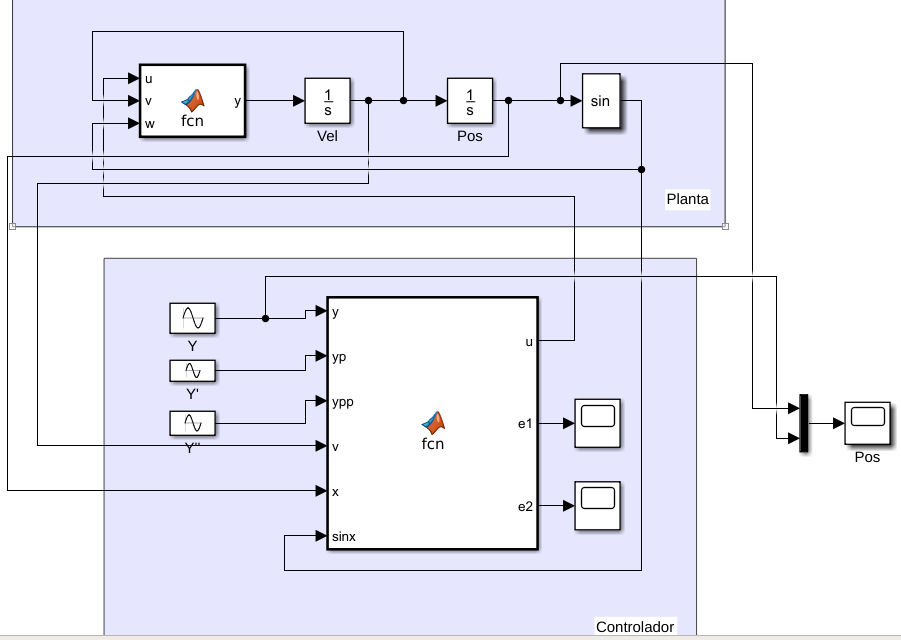
\includegraphics[width=\textwidth]{sysold.png}
	\caption{Sistema dinámico simplficado.}
\end{figure}

En este caso deseamos obtener una perturbación igual a la que teníamos en el sistema dinámico cuando la añadíamos como onda senoidal. Si recordamos, tomamos ventaja del tiempo transcurrido en la simulación para poder añadir la perturbación. Por lo tanto, en este caso será similar, ya que necesitaremos algún tipo de contador para lograr encender y apagar la señal después de cierto tiempo. 

Para esto el reloj analógico nos puede ayudar. Éste funcionará como entrada en ambas funciones, ya que si recordamos, además de tener la peturbación en función del tiempo, las ganancias también solian ser dinámicas. Esto nos lleva a hacer dependientes nuestras ganancias del tiempo, cambiando sus magnitudes a lo largo del tiempo. Teniendo esto en cuenta podemos añadir el reloj analógico como entrada al sistema que estamos modelando.

\begin{figure}[H]
	\centering
	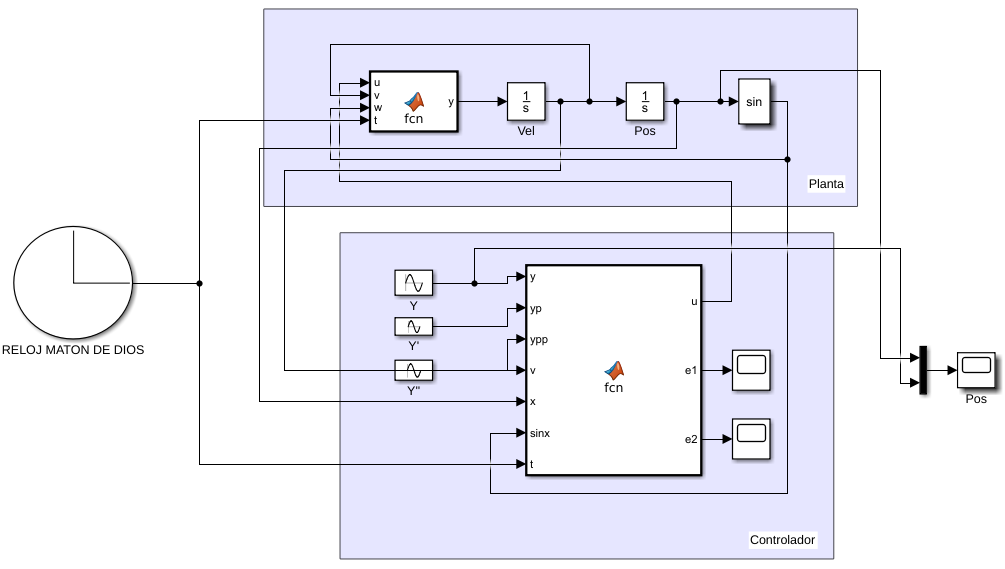
\includegraphics[width=\textwidth]{clock.png}
	\caption{Adición del reloj analógico a las entradas de las funciones.}
\end{figure}

Lo único que nos queda por realizar es modificar el código dentro de las funciones para lograr integrar la variable del tiempo en nuestras entradas y así añadirlas a la ecuación dentro de la función para que nuestra salida sea la deseada, como se muestra a continuación.

\lstinputlisting[style=Matlab-editor, basicstyle=\mlttfamily\scriptsize, caption={Código modificado de la planta.}]{./code/sin.m}

El código de la planta fue modificado de tal manera que el tiempo manipulará el valor de la función trigonométrica que funcionará como nuestra perturbación, es por eso que la variable dentro del seno será el tiempo \textit{t}, y dado que también queremos activar la perturbación sólo en un rango de tiempo, podemos indicar que la función esté activa solamente cuando el tiempo sea menor a cero, logrando así el objetivo que queríamos desde un inicio.

\lstinputlisting[style=Matlab-editor, basicstyle=\mlttfamily\scriptsize, caption={Código modificado del controlador.}]{./code/two.m}

Por otro lado, en el código de la planta tenemos lo mencionado en prácticas anteriores sobre las ganancias dinámicas, eso para mejorar el sistema después de una cantidad de tiempo y lograr apreciar el peso que tienen estas constantes en la estabilidad de nuestro transitorio.

Es por eso que en el código anteriormente mostrado después de una marca de tiempo las constantes cambian repentinamente, para lograr ese cambio similar al que teníamos antes.

\begin{figure}[H]
	\centering
	\begin{subfigure}[b]{0.49\linewidth}
		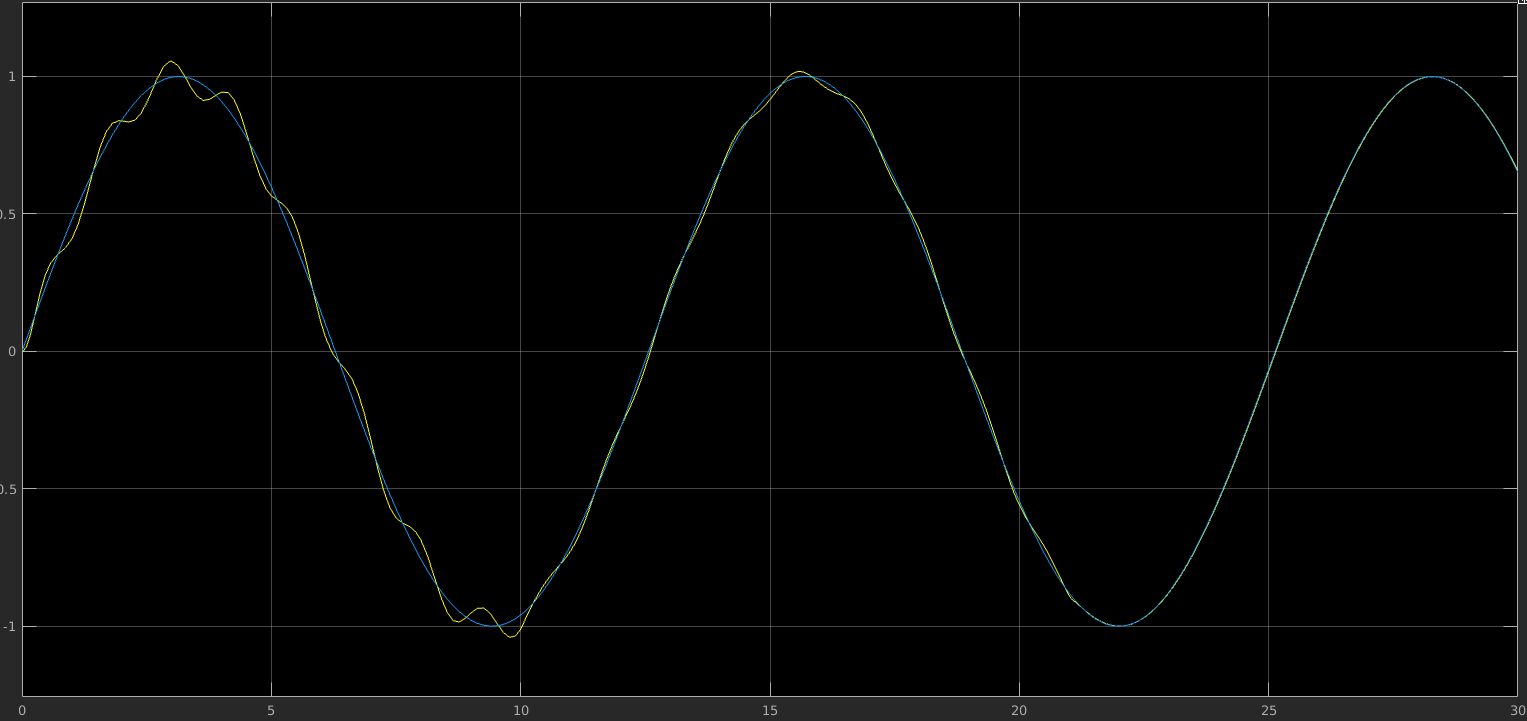
\includegraphics[width=\linewidth]{oldsys.png}
		\caption{Sistema original.}
	\end{subfigure}
	\begin{subfigure}[b]{0.49\linewidth}
		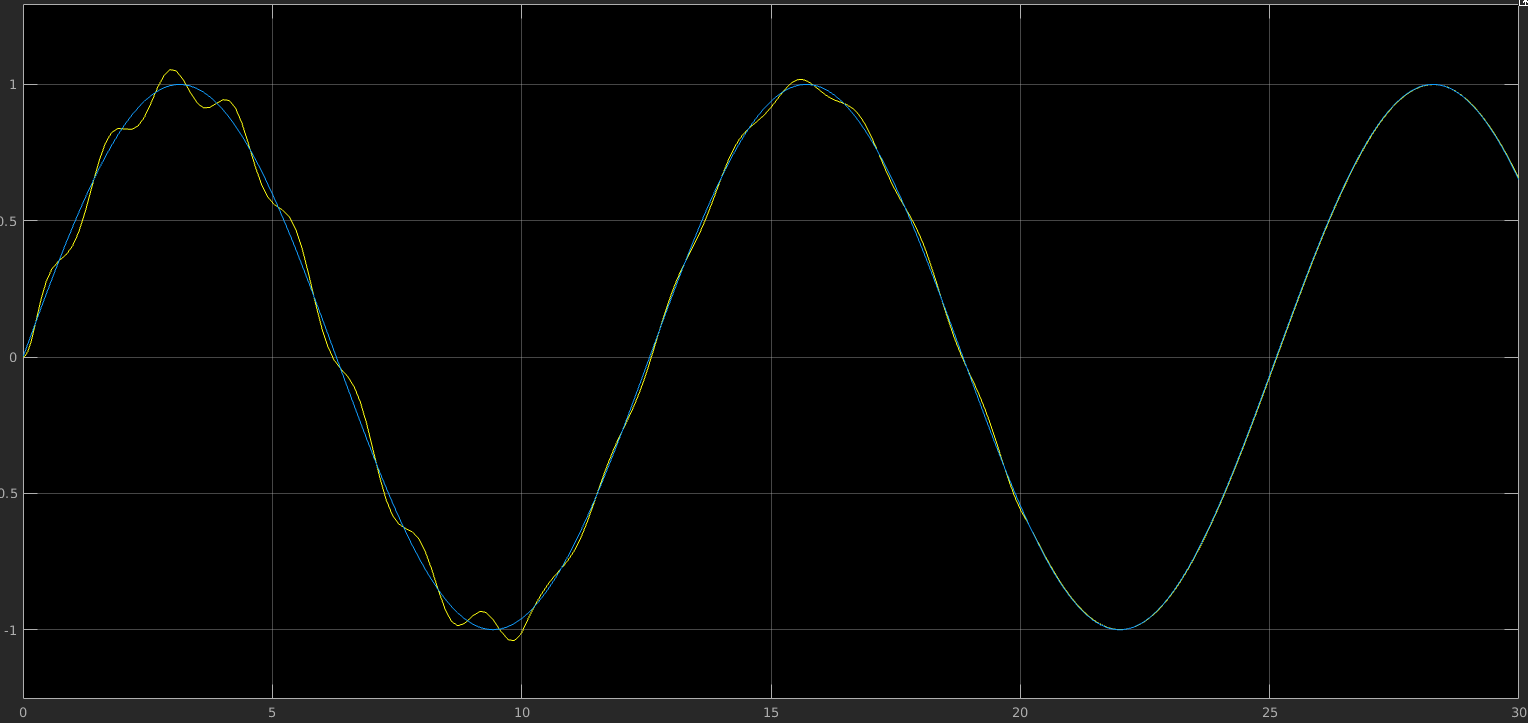
\includegraphics[width=\linewidth]{newsys.png}
		\caption{Sistema nuevo.}
	\end{subfigure}
	\caption{Comparación del sistema original y el sistema expresado en código.}
\end{figure}

Si analizamos las gráficas arrojadas por el sistema original y el sistema nuevo y las comparamos, virtualmente no existe diferencia entre ellas, expresan el mismo sistema de ecuaciones diferenciales y actúan de la misma manera.


\begin{figure}[H]
	\centering
	\begin{subfigure}[b]{0.49\linewidth}
		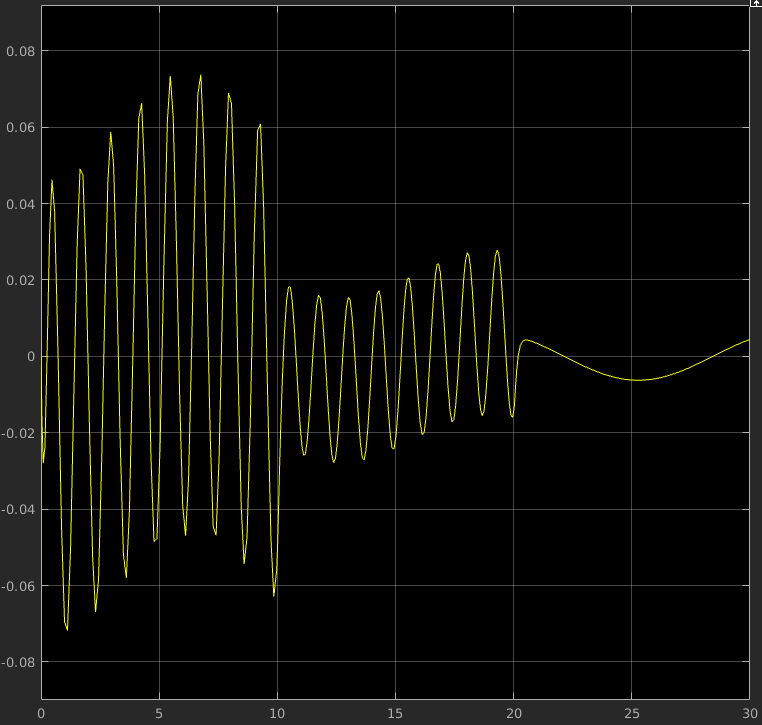
\includegraphics[width=\linewidth]{e1.png}
		\caption{$e_1$}
	\end{subfigure}
	\begin{subfigure}[b]{0.49\linewidth}
		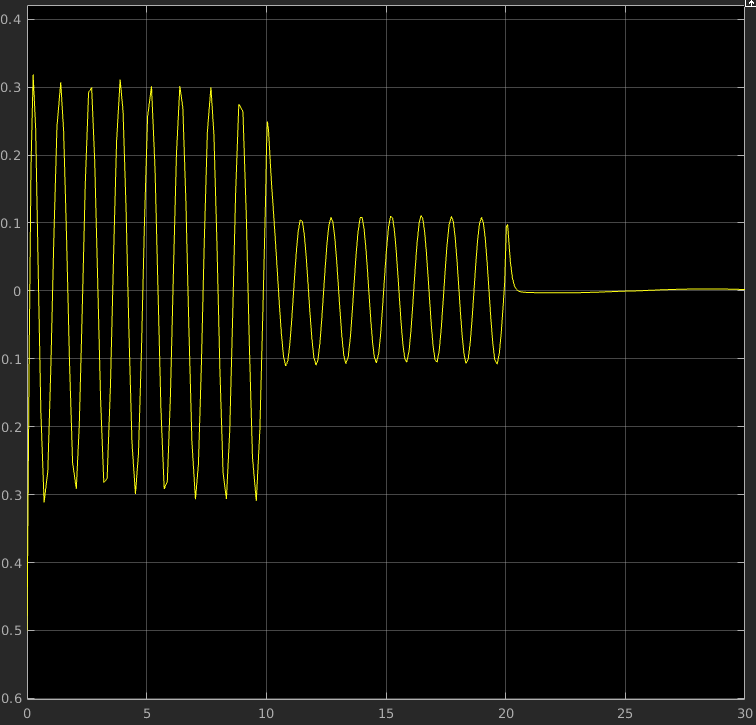
\includegraphics[width=\linewidth]{e2.png}
		\caption{$e_2$}
	\end{subfigure}
	\caption{Errores del sistema actualizado.}
\end{figure}


\begin{figure}[H]
	\centering
	\begin{subfigure}[b]{0.49\linewidth}
		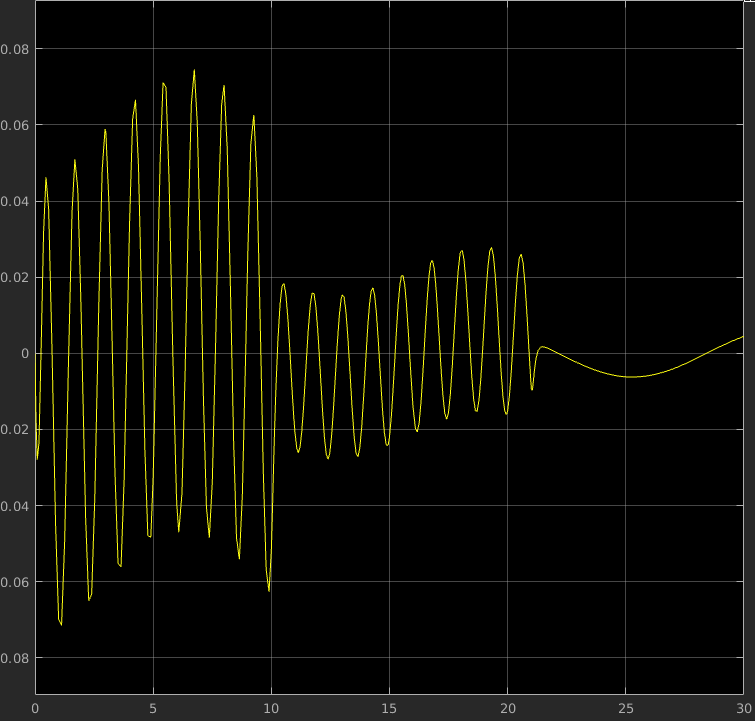
\includegraphics[width=\linewidth]{e1old.png}
		\caption{$e_1$}
	\end{subfigure}
	\begin{subfigure}[b]{0.49\linewidth}
		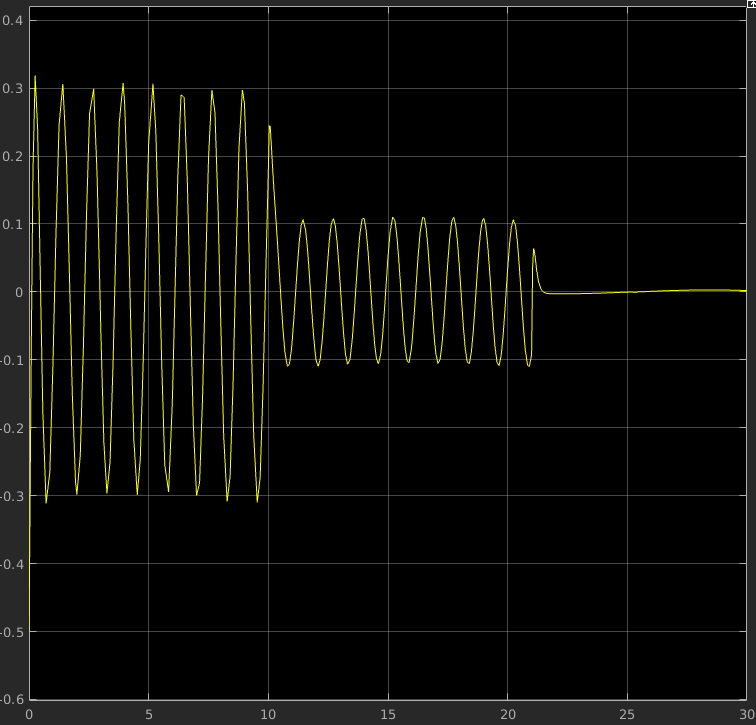
\includegraphics[width=\linewidth]{e2old.png}
		\caption{$e_2$}
	\end{subfigure}
	\caption{Errores del sistema original.}
\end{figure}

\section*{Conclusión}

Como nota final podemos apreciar la facilidad que nos brinda el código para expresar sistemas dinámicos de una manera mucho más sencilla, podemos observar que la diferencia entre los sistemas originales y aquellos actualizados es mínima, sino es que inexistente. 
%%%%%  Bib
\renewcommand\refname{Referencias}
\printbibliography
\end{document}
